\documentclass[10pt,letterpaper]{article}
\usepackage[margin=0.62in]{geometry}
\usepackage{amsmath,amssymb,mathtools,graphicx,booktabs,array,xcolor,fancyhdr,hyperref}
\definecolor{ink}{HTML}{0B3A6B}
\pagestyle{fancy}\fancyhf{}
\fancyhead[L]{\small\sffamily PHYSICS II (CH.\ 25--26) $\cdot$ INTENSIVE REVIEW BLOCK S1}
\fancyhead[R]{\small\sffamily DETAILED WORKED SOLUTIONS}
\fancyfoot[L]{\small\sffamily S2C + Spec v2 MNA Verified $\cdot$ Equivalent Resistance \& Multi-Source KVL/KCL}
\fancyfoot[R]{\small\sffamily\thepage}
\setlength{\headheight}{14pt}\setlength{\parindent}{0pt}\setlength{\parskip}{5pt}
\begin{document}

{\color{ink}\sffamily\bfseries\LARGE Block S1 Solutions: Equivalent Resistance \& Multi-Source KVL/KCL}\par
\textbf{Companion Key to:} \texttt{Block\_S1\_Exercises\_EqResistance\_KVL\_KCL.pdf} \quad|\quad \textbf{MNA Solver Check:} All nodal voltages \& branch currents verified

\section*{Exercise 01 Solutions $\cdot$ First-Principles \& Conical Conductor Calculus Proof \hfill [10 Points]}
\textbf{(a) Series Equivalent Resistance [2 pts]:} In steady state ($\nabla\cdot\mathbf{J}=0$), KCL at each internal junction ensures identical current $I_1 = I_2 = \dots = I_N = I$. Applying KVL ($\sum_{\rm loop}\Delta V=0$), including the source rise, around the loop:
\[
  V_{ab} - \sum_{k=1}^N I R_k = 0 \implies V_{ab} = I \sum_{k=1}^N R_k \implies R_{\text{eq}} = \frac{V_{ab}}{I} = \sum_{k=1}^N R_k. \quad \blacksquare
\]
\textbf{(b) Parallel Equivalent Resistance \& Upper Bound [2 pts]:} The same two nodes enforce identical branch voltage $V_k = V_{ab}$. Applying KCL at node $a$ for $N\ge2$ positive resistors:
\[
  I_{\text{total}} = \sum_{k=1}^N I_k = V_{ab}\sum_{k=1}^N \frac{1}{R_k} \implies \frac{1}{R_{\text{eq}}} = \sum_{k=1}^N \frac{1}{R_k} = \frac{1}{R_{\min}} + \sum_{k\neq\min}\frac{1}{R_k} > \frac{1}{R_{\min}} \implies R_{\text{eq}} < R_{\min}. \quad \blacksquare
\]
\textbf{(c) Continuous Tapered Conical Conductor [6 pts]:} These results are exact within the stated one-dimensional equipotential-slice model; a physical tapered conductor can have spreading fields.
\begin{enumerate}
  \item[(i)] $r(x) = a + \frac{b-a}{L}x$, \quad $A(x) = \pi\left[a + \frac{b-a}{L}x\right]^2$, \quad $dR = \dfrac{\rho\,dx}{\pi\left[a + \frac{b-a}{L}x\right]^2}$.
  \item[(ii)] With $u = a + \frac{b-a}{L}x$ and $dx = \frac{L}{b-a}\,du$:
  \[
    R = \frac{\rho L}{\pi(b-a)}\int_a^b u^{-2}\,du = \frac{\rho L}{\pi(b-a)}\left(\frac{1}{a}-\frac{1}{b}\right) = \frac{\rho L}{\pi a b}.
  \]
  \item[(iii)] As $b \to a$, $R \to \frac{\rho L}{\pi a^2} = \frac{\rho L}{A}$. Inside the frustum, $E(x) = \rho J(x) = \dfrac{\rho I}{\pi[a + (b-a)x/L]^2}$.
\end{enumerate}

\section*{Exercise 02 Solutions $\cdot$ Mixed Series--Parallel DC Ladder \hfill [10 Points]}
\begin{enumerate}
  \item[(a)] $R_{34} = R_3 + R_4 = 4.00 + 5.00 = 9.00\ \Omega$; \quad $R_{BG} = \frac{(18.0)(9.00)}{18.0+9.00} = 6.00\ \Omega$; \quad $R_{\text{eq}} = R_1 + R_{BG} = 6.00 + 6.00 = 12.0\ \Omega$.
  \item[(b)] $I_{\text{src}} = \frac{36.0}{12.0} = 3.00\text{ A}$; \quad $V_B = 36.0 - (3.00)(6.00) = 18.0\text{ V}$; \quad $I_2 = \frac{18.0}{18.0} = 1.00\text{ A}$; \quad $I_{34} = \frac{18.0}{9.00} = 2.00\text{ A}$; \quad $V_D = I_{34}R_4 = 10.0\text{ V}$.
  \item[(c)] $P_{R_1}=54.0\text{ W}$, $P_{R_2}=18.0\text{ W}$, $P_{R_3}=16.0\text{ W}$, $P_{R_4}=20.0\text{ W}$; \quad $\sum P_{R_k} = 108.0\text{ W} = (36.0\text{ V})(3.00\text{ A})$.
  \item[(d)] Shorting $R_3 \to 0$: $R_{BG}' = \frac{(18.0)(5.00)}{23.0} = \frac{90}{23}\ \Omega \approx 3.913\ \Omega$, \quad $R_{\text{eq}}' = \frac{228}{23} \approx 9.91\ \Omega$, \quad $I_{\text{src}}' = \frac{69}{19} \approx 3.63\text{ A}$, \quad $V_B' = \frac{270}{19} \approx 14.21\text{ V}$, \quad $P_{R_4}' = \frac{(V_B')^2}{5.00} \approx 40.4\text{ W}$ ($2.02\times$ increase).
\end{enumerate}

\section*{Exercise 03 Solutions $\cdot$ Multi-Source KVL/KCL Network \hfill [12 Points]}
\begin{enumerate}
  \item[(a)] KCL at $A$: $I_1 + I_2 + I_3 = 0$. Left mesh KVL: $+18.0 + 3.00 I_1 - 6.00 I_2 = 0$. Right mesh KVL: $+6.00 I_2 - 3.00 I_3 - 9.00 = 0$.
  \item[(b)] Nodal KCL: $\frac{V_A - 18.0}{3.00} + \frac{V_A}{6.00} + \frac{V_A - 9.00}{3.00} = 0 \implies 5V_A = 54.0 \implies V_A = 10.8\text{ V}$. Thus $I_1 = -2.40\text{ A}$ ($2.40\text{ A}$ upward), $I_2 = +1.80\text{ A}$ (downward), $I_3 = +0.600\text{ A}$ (downward).
  \item[(c)] $\mathcal{E}_1$ delivers $P_{\mathcal{E}_1} = (18.0)(2.40) = 43.2\text{ W}$. $\mathcal{E}_3$ absorbs $P_{\mathcal{E}_3} = (9.00)(0.600) = 5.40\text{ W}$. Net delivered $= 37.8\text{ W} = 17.28 + 19.44 + 1.08 = \sum I_k^2 R_k$.
\end{enumerate}

\section*{Exercise 04 Solutions $\cdot$ Cloze \& Maximum Power Transfer \hfill [10 Points]}
\textbf{Part A Key:} (a) \texttt{electric charge}, (b) \texttt{energy}, (c) \texttt{smaller than}, (d) \texttt{opposite to}, (e) $\mathcal{E}-Ir$, (f) $\mathcal{E}+Ir$, (g) \texttt{open circuit}, (h) \texttt{short circuit}.\par
\textbf{Part B Proof:} $P_L(R_L) = \frac{\mathcal{E}^2 R_L}{(r+R_L)^2} \implies \frac{dP_L}{dR_L} = \mathcal{E}^2\frac{r-R_L}{(r+R_L)^3} = 0 \implies R_L = r = 3.00\ \Omega$, $P_{L,\max} = \frac{\mathcal{E}^2}{4r} = 27.0\text{ W}$.
\begin{center}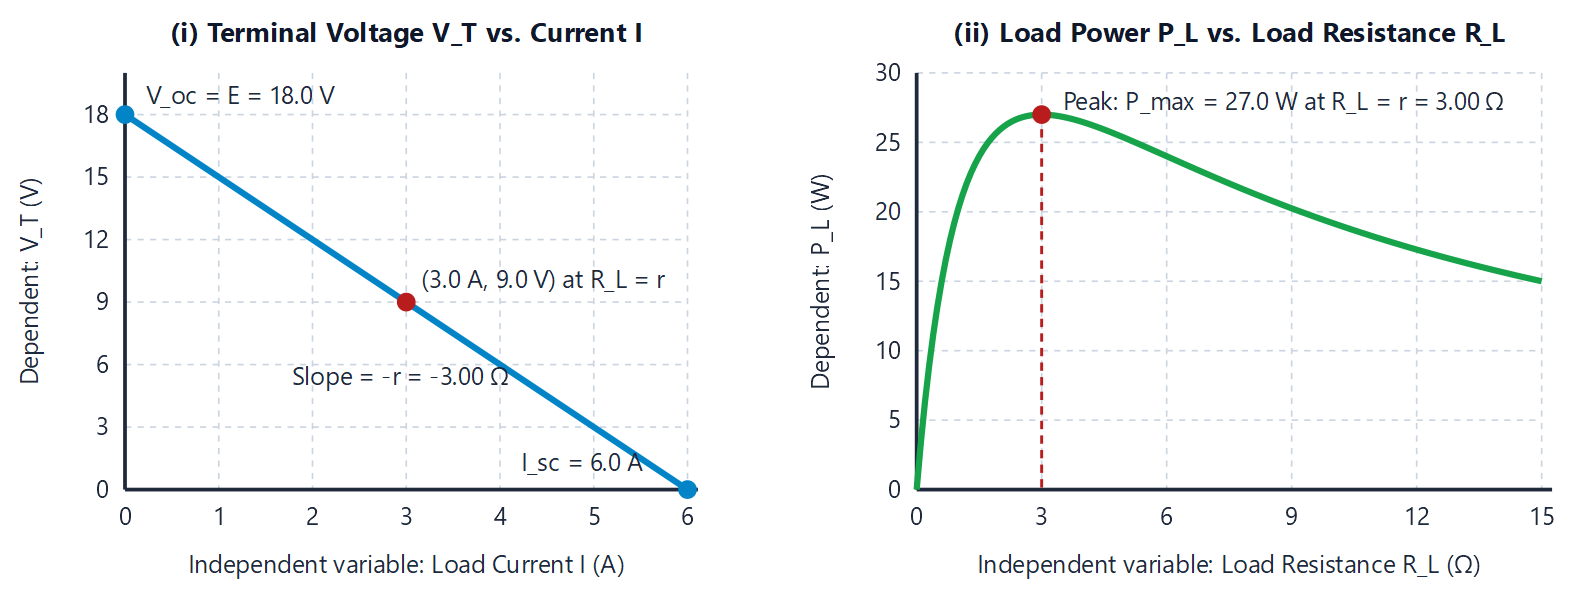
\includegraphics[width=0.92\linewidth]{block_s1_assets/s1-q4-grid-solved.png}\end{center}
\end{document}
